%!TEX root = /Users/ede/Documents/Master/19_AS/Ausarbeitung/as-ausarbeitung.tex
\section{Analyse und Klassifikation} % (fold)
\label{sec:analyse_und_klassifikation}

Um die Tag-Rankingverfahren hinsichtlich der oben genannten Anwendungsgebiete zu formulieren und zu optimieren, müssen zunächst die vorhandenen Tags in einer Folksonomy analysiert werden \cite{collectiveKnowledge}. Als Datenbasis aller vorgestellten Ansätze dient die Fotocommunity Flickr.

%TODO: mehr beschreiben, wofür die Analyse und Klassifikation benötigt wird, und was als Ergbenis erwartet wird(z.B. Dass folgende Fragen beantwortet werden)

Folgende Fragen stellen sich hierbei:
\begin{itemize}
	\item     Welche Tags sind vorhanden?
	\item     Wie gehen Benutzer beim Taggen vor?
	\item     In welcher Reihenfolge liegen die Tags vor?
	\item     In welchen Beziehungen stehen die Tags untereinander?
	\item     In wie weit gleicht der Inhalt der Photos, wenn gleiche Tags vorhanden sind?
	\item     Können die Tags in Kategorien zusammengefasst werden?
\end{itemize}


\subsection{Analyse der Tags und Photos} % (fold)
\label{sub:analyse_der_tags}

 \begin{itemize}
  \item Frequenz der Tags, Viele Tags werden sehr selten benutzt
  \item Anzahl der Tags pro Photo
  \item Position der relevanten Tags
 \begin{figure}[htbp]
    \centering
      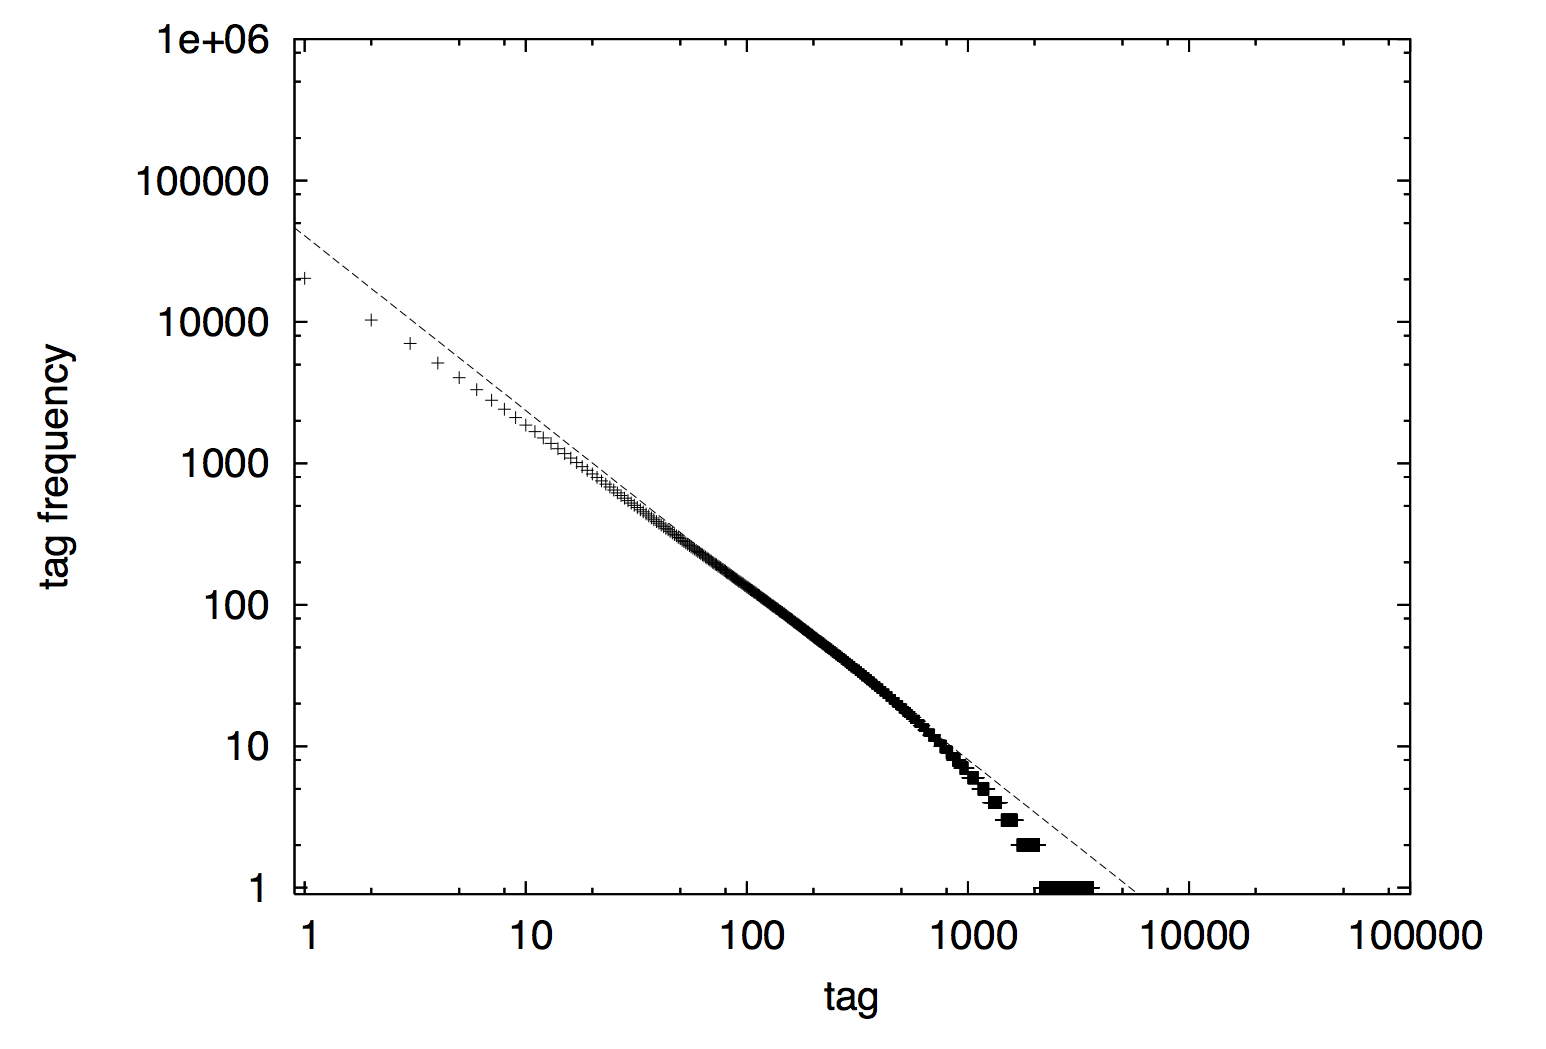
\includegraphics[height=3in]{images/collectiveKnowledge_tag_frequency.png}
    \caption{Distribution of the Tag Frequency in Flickr aus \cite{collectiveKnowledge}}
    \label{fig:images_collectiveKnowledge_word_net_categories}
  \end{figure}
  
  \begin{figure}[htbp]
    \centering
      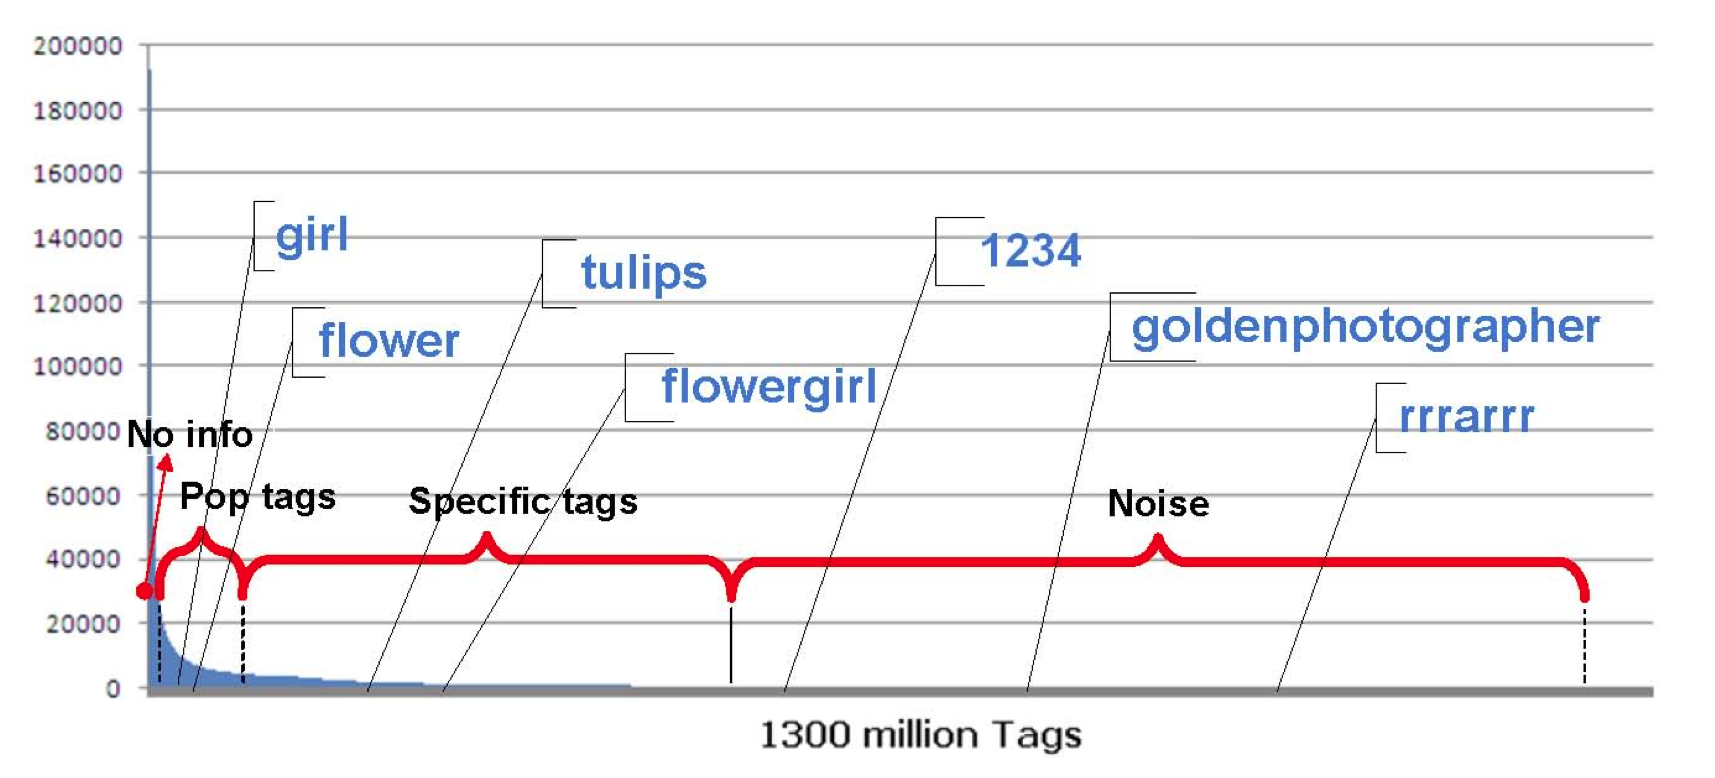
\includegraphics[height=3in]{images/learning_to_tag_frequency.png}
    \caption{Tag distribution over a collection of 640 million images from Flickr.com. There are totally 1,300 million tags. Around 1\% of the tags appearing more than 20,000 times, which contain little information. Around 5.82\% of the tags have appeared more than 5,000 in the collection, which are considered as popular tags. 33.21\% of the tags appears more than 50 and less than 5,000 times, which are defined as specific tags. 60\% of the tags have appeared less than 50 times, aus \cite{learningToTag}}
    \label{fig:images_learning_to_tag_frequency}
  \end{figure}
  
  
  \begin{figure}[htbp]
    \centering
      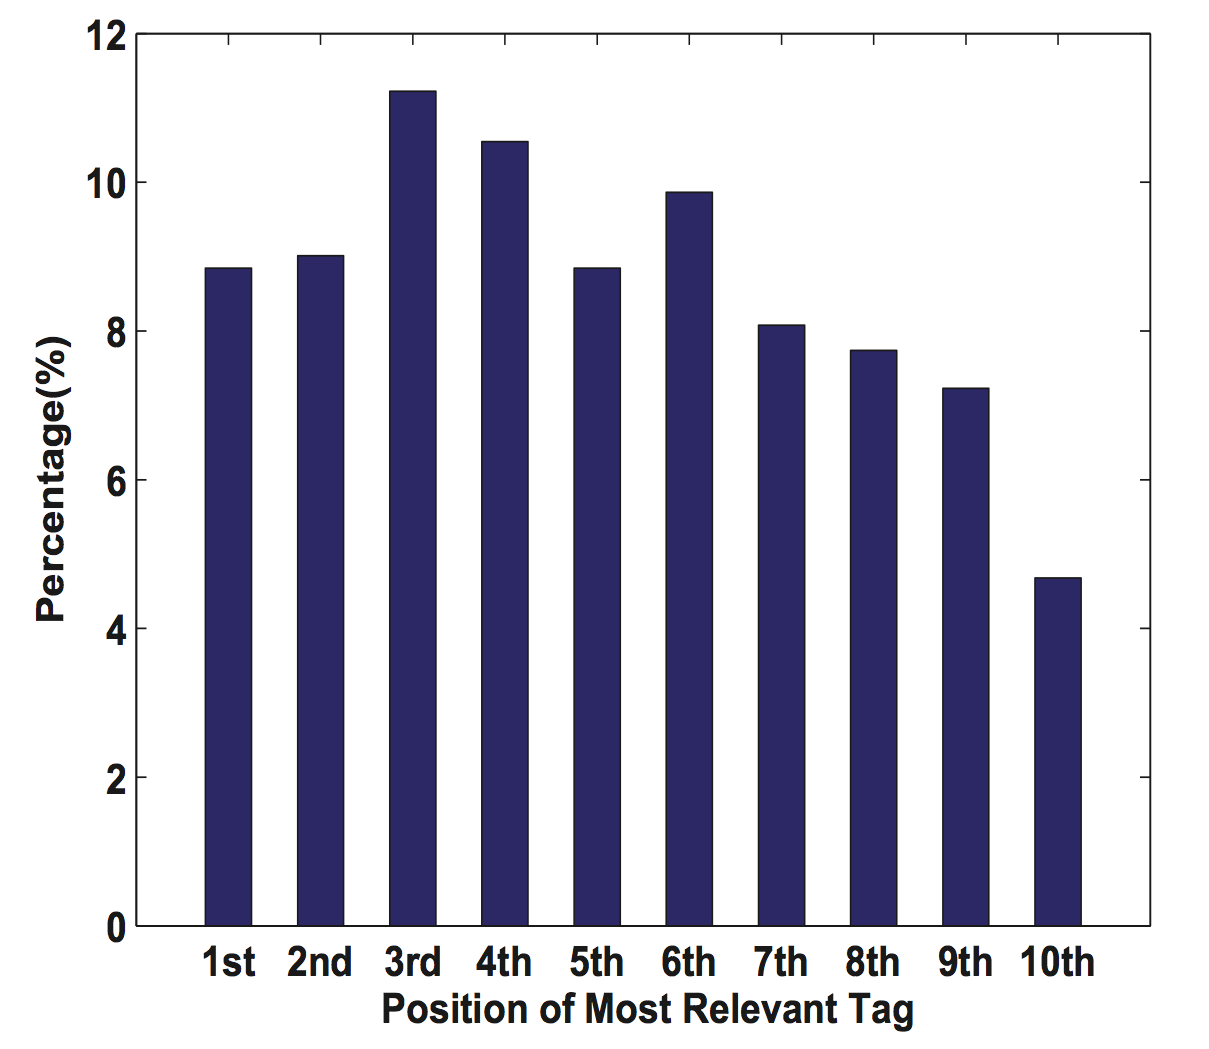
\includegraphics[height=3in]{images/tag_ranking_psotion_relevant_tag.png}
    \caption{Percentage of images that have their most relevant tag at the n-th position in the associated tag list, where n = 1,2,3...,10. Aus \cite{ranking}}
    \label{fig:images_tag_ranking_psotion_relevant_tag}
  \end{figure}
  
  
 \end{itemize}
% subsection analyse_der_tags (end)

\subsection{Klassifikation von Tags und Photos} % (fold)
\label{sub:klassifikation_von_tags}

\cite{collectiveKnowledge} untersuchten 52 Millionen Photos und deren Tags aus Flickr. Für die Photos wurde eine Klassifizierung nach der Anzahl gesetzter Tags gewählt. Diese Klassen finden später noch in der Evaluation der Leistung des verwendeten Verfahrens Einsatz.

\begin{tabular}{ccc}
\hline
 & Tags per photo & Photos\\
\hline
Class I & 1 & ca. 15,5 Millionen\\
\hline
Class II & 2 - 3 & ca. 17,5 Millionen\\
\hline
Class III & 4 - 6 & ca. 12 Millionen\\
\hline
Class IV & > 6 & ca. 7 Millionen\\
\hline
\end{tabular}

\subsubsection*{Tags} % (fold)
\label{ssub:tags}

% subsubsection tags (end)  
\cite{collectiveKnowledge}: 
- To answer the question “What are users tagging?”, we have mapped Flickr tags onto the WordNet broad categories, siehe Abbildung \ref{fig:collectiveKnowledge_word_net_categories}

\begin{figure}[htbp]
  \centering
    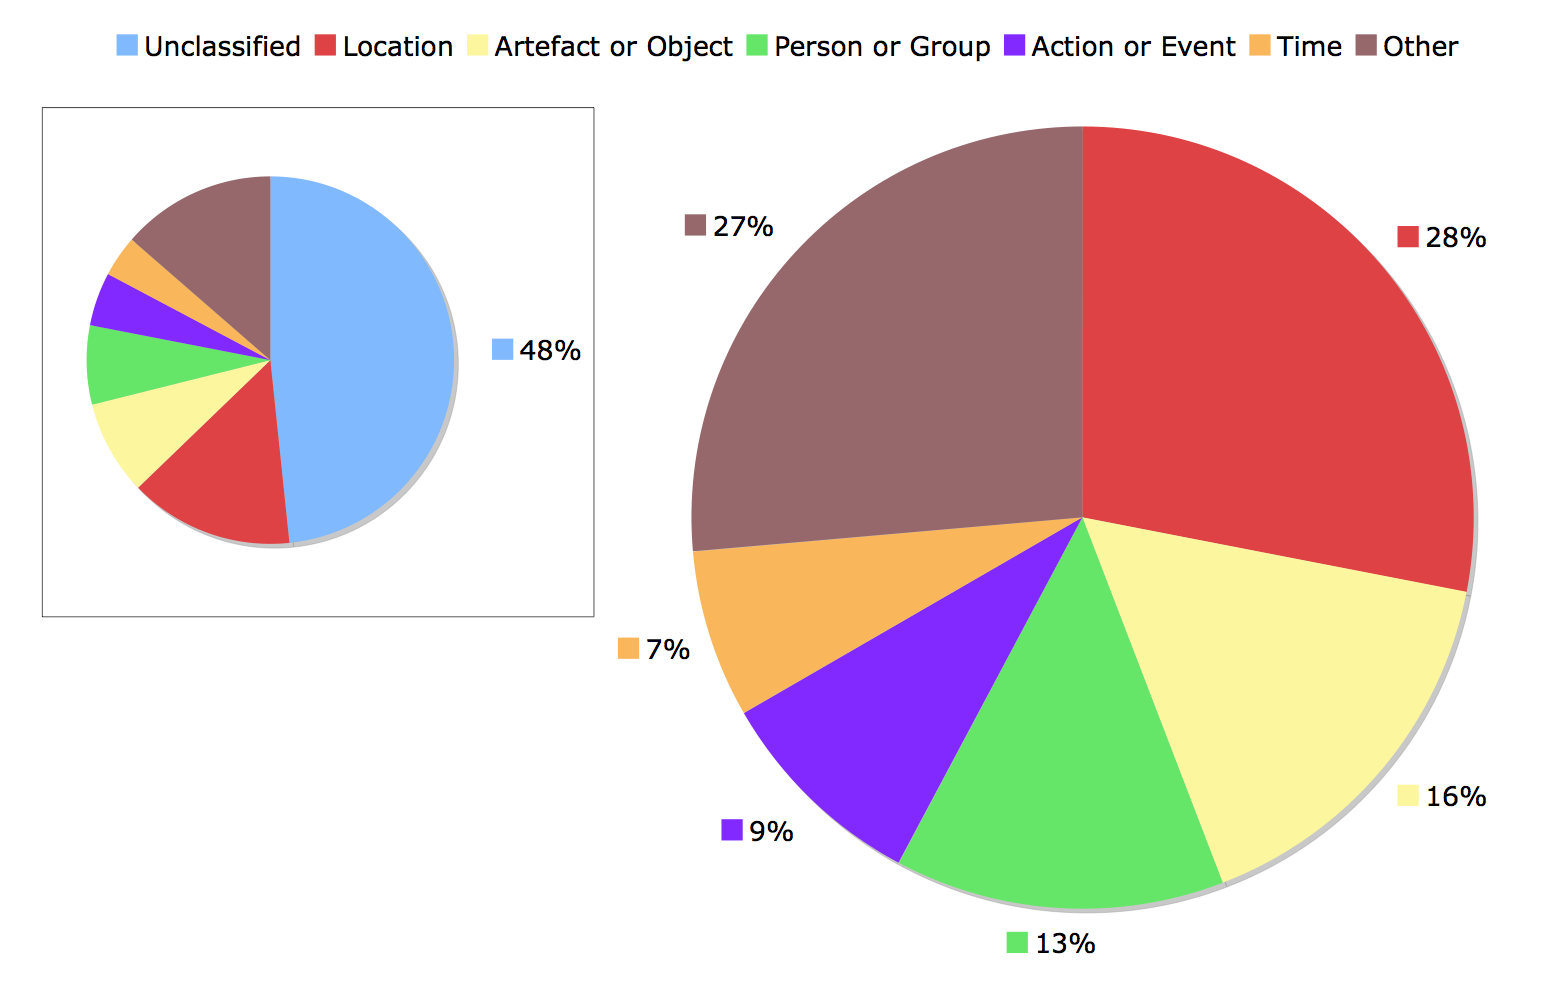
\includegraphics[height=3in]{images/collectiveKnowledge_word_net_categories.png}
  \caption{Most frequent WordNet categories for Flickr tags aus \cite{collectiveKnowledge}}
  \label{fig:collectiveKnowledge_word_net_categories}
\end{figure}


- To analyse the behaviour of the tag recommendation systems for photos with dierent levels of exhaustiveness of the original annotation

- From this information, we can conclude that users do not only tag the visual contents of the photo, but to a large extent provide a broader context in which the photo was taken, such as, location, time, and actions.

Damit ist auch geklärt, welche Art von Tags Benutzer am häufigsten verwenden. Auf Basis dieser Analyse und Klassifikation wurde das Verfahren entwickelt, welches in Abschnitt \ref{sec:tag_ranking_verfahren} beschrieben wird.


% subsection klassifikation_von_tags (end)




% section analyse_und_klassifikation (end)
